Nach erfolgreicher Einrichtung einer Cloud Node im Spectrum Scale Cluster, kann diese nun mit unterschiedlichen Cloud Speichern verbunden werden.

Bei der Einrichtung wird davon ausgegangen, dass folgende Einstellungen vorgenommen wurden:
\begin{itemize}
	\item Name der NodeClass: \textbf{TCTNodeClass}
	\item Cloud Typ: \textbf{mcstore}
	\item Name des Cloud-Dateisystems: \textbf{fs1}
\end{itemize}

Nach Hochfahren des Clusters kann mit \lstinline|mmhealth node show|, der Status der unterschiedlichen Dienste untersucht werden. Auf einer einzelnen Maschine kann es aber einige Minuten bauen, bis Scale vollständig hochgefahren ist.

Um den Zustand des Cloud Dienstes zu inspizieren, mit ihm zu arbeiten (Datei Sharing / Tiering) oder ihn zu verändern wird das \lstinline|mmcloudgateway| Programm verwendet. Falls dieser nicht automatisch beim Systemstart initialisiert wird, kann er mithilfe von \lstinline|mmcloudgateway service start -N TCTNodeClass| manuell gestartet werden.

\begin{figure}[hbt]
	\centering
	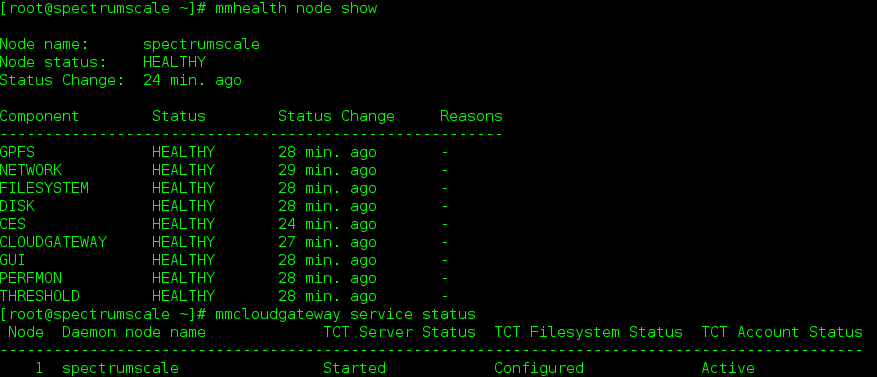
\includegraphics[scale=0.5]{images/scale-status}
	\caption{Beispielhafte Ausgabe von \lstinline|mmhealth| und \lstinline|mmcloudgateway| - mit konfiguriertem Cloudgateway}
	\label{fig:saclestatus}
\end{figure}


\textbf{Einrichtung des Cloud Sharing Accounts}\\
Nun muss zuerst die S3 Verbindung mit \ac{COS} hergestellt werden. Dafür sollte ein Test der Account Daten im Vorhinhein stattfinden, um spätere Probleme bei der Einrichtung verhindern.

Ein IBM Cloud Object Storage Account auf Softlayer kann unter dieser URL \url{https://www.ibm.com/cloud-computing/bluemix/cloud-object-storage} eingerichtet werden. 

Nach erfolgreicher Erstellung kann ein erster Bucket erstellt und Nutzername, Adresse des Endpunkts und Passwort ausgelesen werden. Hierbei gibt es Unterschiede bei der Befehl Syntax zwischen Spectrum Scale und \ac{COS}. 
Der Nutzername wird bei S3 kompatiblen Schnittstellen normalerweise als \textit{AccessKeyId} und das Passwort als \textit{SecretAccessKey} bezeichnet.\\

\begin{lstlisting}[language=bash, caption=Vortest des Cloud Sharing Accounts]
mmcloudgateway account pre-test --cloud-type cleversafe-new --username "<username>" --pwd-file <path/file/your/secretAccessKey> --cloud-url <cos/endpoint>
\end{lstlisting}

Nach Ausführung wird eine Testverbindung aufgebaut, entstehen keine Fehlermeldungen kann nun der Account eingerichtet werden. An dieser Stelle ist es extrem wichtig, dass die Option \lstinline|--enc-enable| auf \lstinline|FALSE| gesetzt wird. Ansonsten kann das beabsichtigte Cloud Sharing nicht umgesetzt werden, da beim Export eine Dateiverschlüsselung stattfindet. Diese macht das Lesen der Informationen von anderen Anwendungen (hier unsere Demoanwendung) unmöglich.

Die Befehlssyntax benötigt an dieser Stelle aber noch weitere Informationen, die für deinen eigentlichen Test nicht notwendig waren:\\

\begin{lstlisting}[language=bash, caption=Einrichtung des Cloud Sharing Accounts]
mmcloudgateway account create --cloud-nodeclass TCTNodeClass --cloud-name mcstore --cloud-type cleversafe-new --username "<username>" --pwd-file <path/file/your/secretAccessKey> --enable TRUE --cloud-url <cos/endpoint> --enc-enable FALSE
\end{lstlisting}

Nach erfolgreicher Ausführung des Befehls ist der Account fertig eingerichtet und man sollte folgende Ausgabe (\autoref{fig:saclestatus}) bei dem Überprüfen des Cloud Services sehen.

\textbf{Export von lokalen Dateien in die Cloud}\\
Um Informationen in den konfigurierten Cloud Account zu exportieren, muss zuerst in das ausgewählte Datei System für die Cloud Knoten gewechselt werden (hier: \lstinline|cd /gpfs/fs1|).

Mit dem bereits bekannten \lstinline|mmcloudgateway| Befehl können nun einzelne oder mehrere Files zwischen \ac{COS} und der lokalen Maschine kopiert werden.

Es besteht die Möglichkeit Metadaten beim Sharing zu erhalten und alle exportierten Files können in einem Manifest festgehalten werden. Dieses hilft beim späteren Import, da eine List alle exportierten Dateien vorliegt. 

\begin{lstlisting}[language=bash, caption=Export von lokalen Dateien]
mmcloudgateway files export <path/to/file> --manifest-file manifest.txt --export-metadata
\end{lstlisting}

\begin{lstlisting}[language=bash, caption=Import von COS Dateien]
mmcloudgateway files import <fileKey> --import-metadata
\end{lstlisting}

Weitere Informationen hierzu befinden sich in \cite[S. 613]{scale.2017}.

\textbf{Erweiterung der Spectrum Scale Funktionalität}\\
Da Spectrum Scale keinerlei Kontrolle über die geteilten Daten hat, wird es auch nicht über mögliche neue Dateien informiert. Diese können also nativ nicht wieder importiert werden, da keine Informationen vorliegen.

Um dies zu umgehen, gibt es zwei Möglichkeiten: Es kann ein kleiner Webserver auf einem Spectrum Scale Knoten aufgesetzt werden, der von außen über Änderungen informiert wird und diese dann in das Manifest schreibt. Nachteil an dieser Lösung ist, dass zusätzliche Software für Scale entwicklet werden muss und diese auch immer nur auf einem Knoten läuft, was zu Leistungsengpässen führen kann.

Alternativ kann die Manifest Datei auch mit in den Cloudspeicher hochgeladen werden. Von hier kann eine Aktualisierung durch die Cloudanwendung (\autoref{sec:application}) geschehen, jedes Mal wenn neue Daten hinzugefügt werden. Spectrum Scale kann nun immer als erstes die Manifest Datei wieder importieren und bekommt mit dieser dann Information über die Dateiveränderung.

Offensichtlich ist zweite Lösung besser, da keine Veränderung am Cluster vorgenommen werden muss.